\documentclass[a4paper,oneside,12pt]{extreport}

\usepackage{mmap}
\usepackage[T2A]{fontenc}
\usepackage[utf8]{inputenc}
\usepackage[english,russian]{babel}

\usepackage[left=30mm, right=15mm, top=20mm, bottom=20mm]{geometry}

\setlength{\parindent}{1.25cm} % Абзацный отступ

\usepackage{setspace}
\onehalfspacing % Полуторный интервал

\frenchspacing % Равномерные пробелы
\usepackage{indentfirst} % Красная строка

\usepackage{microtype}
\sloppy

\usepackage{titlesec}
\titlespacing*{\chapter}{0pt}{-30pt}{8pt}
\titlespacing*{\section}{\parindent}{*4}{*4}
\titlespacing*{\subsection}{\parindent}{*4}{*4}
\titleformat{\chapter}{\LARGE\bfseries}{\thechapter}{20pt}{\LARGE\bfseries}
\titleformat{\section}{\Large\bfseries}{\thesection}{40pt}{\Large\bfseries}

\usepackage{graphicx}
\usepackage{caption}

\usepackage[unicode,pdftex]{hyperref}
\hypersetup{hidelinks}

\usepackage{amsmath}

%% title begin
\usepackage{wrapfig}

\makeatletter
	\def\vhrulefill#1{\leavevmode\leaders\hrule\@height#1\hfill \kern\z@}
\makeatother
%% title end

%% begin code
\usepackage{listings}
\usepackage{xcolor}

\lstset{
	basicstyle=\footnotesize\ttfamily,
	breakatwhitespace=true,
	breaklines=true,
	commentstyle=\color{gray},
	frame=single,
	keywordstyle=\color{blue},
	stringstyle=\color{red},
	tabsize=8
}

\newcommand{\code}[1]{\texttt{#1}}
%% end code


\begin{document}

\begin{titlepage}
	{\large % 14pt instead of 12pt
	\onehalfspacing
	\centering

	\begin{wrapfigure}[7]{l}{0.14\linewidth}
		\vspace{3mm}
		\hspace{-10mm}
		
\includegraphics[width=0.93\linewidth]{inc/img/bmstu-logo}
	\end{wrapfigure}
	{\singlespacing \footnotesize \bfseries Министерство науки и высшего образования Российской Федерации\\Федеральное государственное бюджетное образовательное учреждение\\высшего образования\\<<Московский государственный технический университет\\имени Н.~Э.~Баумана\\ (национальный исследовательский университет)>>\\(МГТУ им. Н.~Э.~Баумана)\\}

	\vspace{-2.2mm}
	\vhrulefill{0.9mm}\\
	\vspace{-7.5mm}
	\vhrulefill{0.2mm}\\
	\vspace{2mm}

	{\doublespacing \small \raggedright ФАКУЛЬТЕТ \hspace{37mm} «Информатика и системы управления»\\
	КАФЕДРА \hspace{17mm} «Программное обеспечение ЭВМ и информационные технологии»\\}

	\vspace{30mm}

	\textbf{ОТЧЁТ}\\
	По лабораторной работе № 2\\
	По курсу: «Моделирование»\\
	Тема: «Распределение случайных величин»\\
	Вариант: 6 $\equiv$ 2 (mod 4)\\

	\vspace{40mm}

	\begin{flushleft}
		\begin{tabular}{lr}
			\textbf{Студент:}        & Керимов~А.~Ш. \\
			\textbf{Группа:}         & ИУ7-74Б       \\
			\textbf{Оценка (баллы):} & \hrulefill    \\
			\textbf{Преподаватель:}  & Рудаков~И.~В. \\
		\end{tabular}
	\end{flushleft}

	\vfill

	Москва\\
	\the\year\\}
\end{titlepage}

\setcounter{page}{2}


\tableofcontents

\chapter{Теоретическая часть}

\section{Вихрь Мерсенна}

В качестве генератора псевдослучайных чисел был выбран вихрь Мерсенна, а именно вариант MT19937 с периодом $2^{19937} - 1$, поставляемый \href{https://en.cppreference.com/w/cpp/numeric/random/mersenne_twister_engine}{стандартной библиотекой языка C++}.

Алгоритм основывается на свойствах простых чисел Мерсенна и обеспечивает быструю генерацию высококачественных по критерию случайности псевдослучайных чисел.

Вихрь Мерсенна лишён многих недостатков, присущих другим ГПСЧ, таких как малый период, предсказуемость, легко выявляемые статистические закономерности.

\section{Табличный метод}

Табличные генераторы в качестве источника случайных чисел используют специальным образом составленные таблицы, содержащие проверенные некоррелированные цифры.

Табличный генератор случайных чисел в лабораторной работе использует таблицу из книги «\href{https://www.rand.org/pubs/monograph_reports/MR1418.html}{A Million Random Digits with 100,000 Normal Deviates}».

\section{Критерий равномерности}

В качестве критерия равномерности был выбран критерий серий.

Пусть имеется последовательность целых чисел $\left<X_{2n}\right> = X_0, X_1, \ldots, X_{2n - 1}$, элементы которого, как предполагается, независимы и распределены между $0$ и $d - 1$.
Требование, предъявляемое к этой последовательности, состоит в следующем: пары последовательных чисел должны быть распределены независимо и равномерно.

\begin{figure}[H]
	\centering
	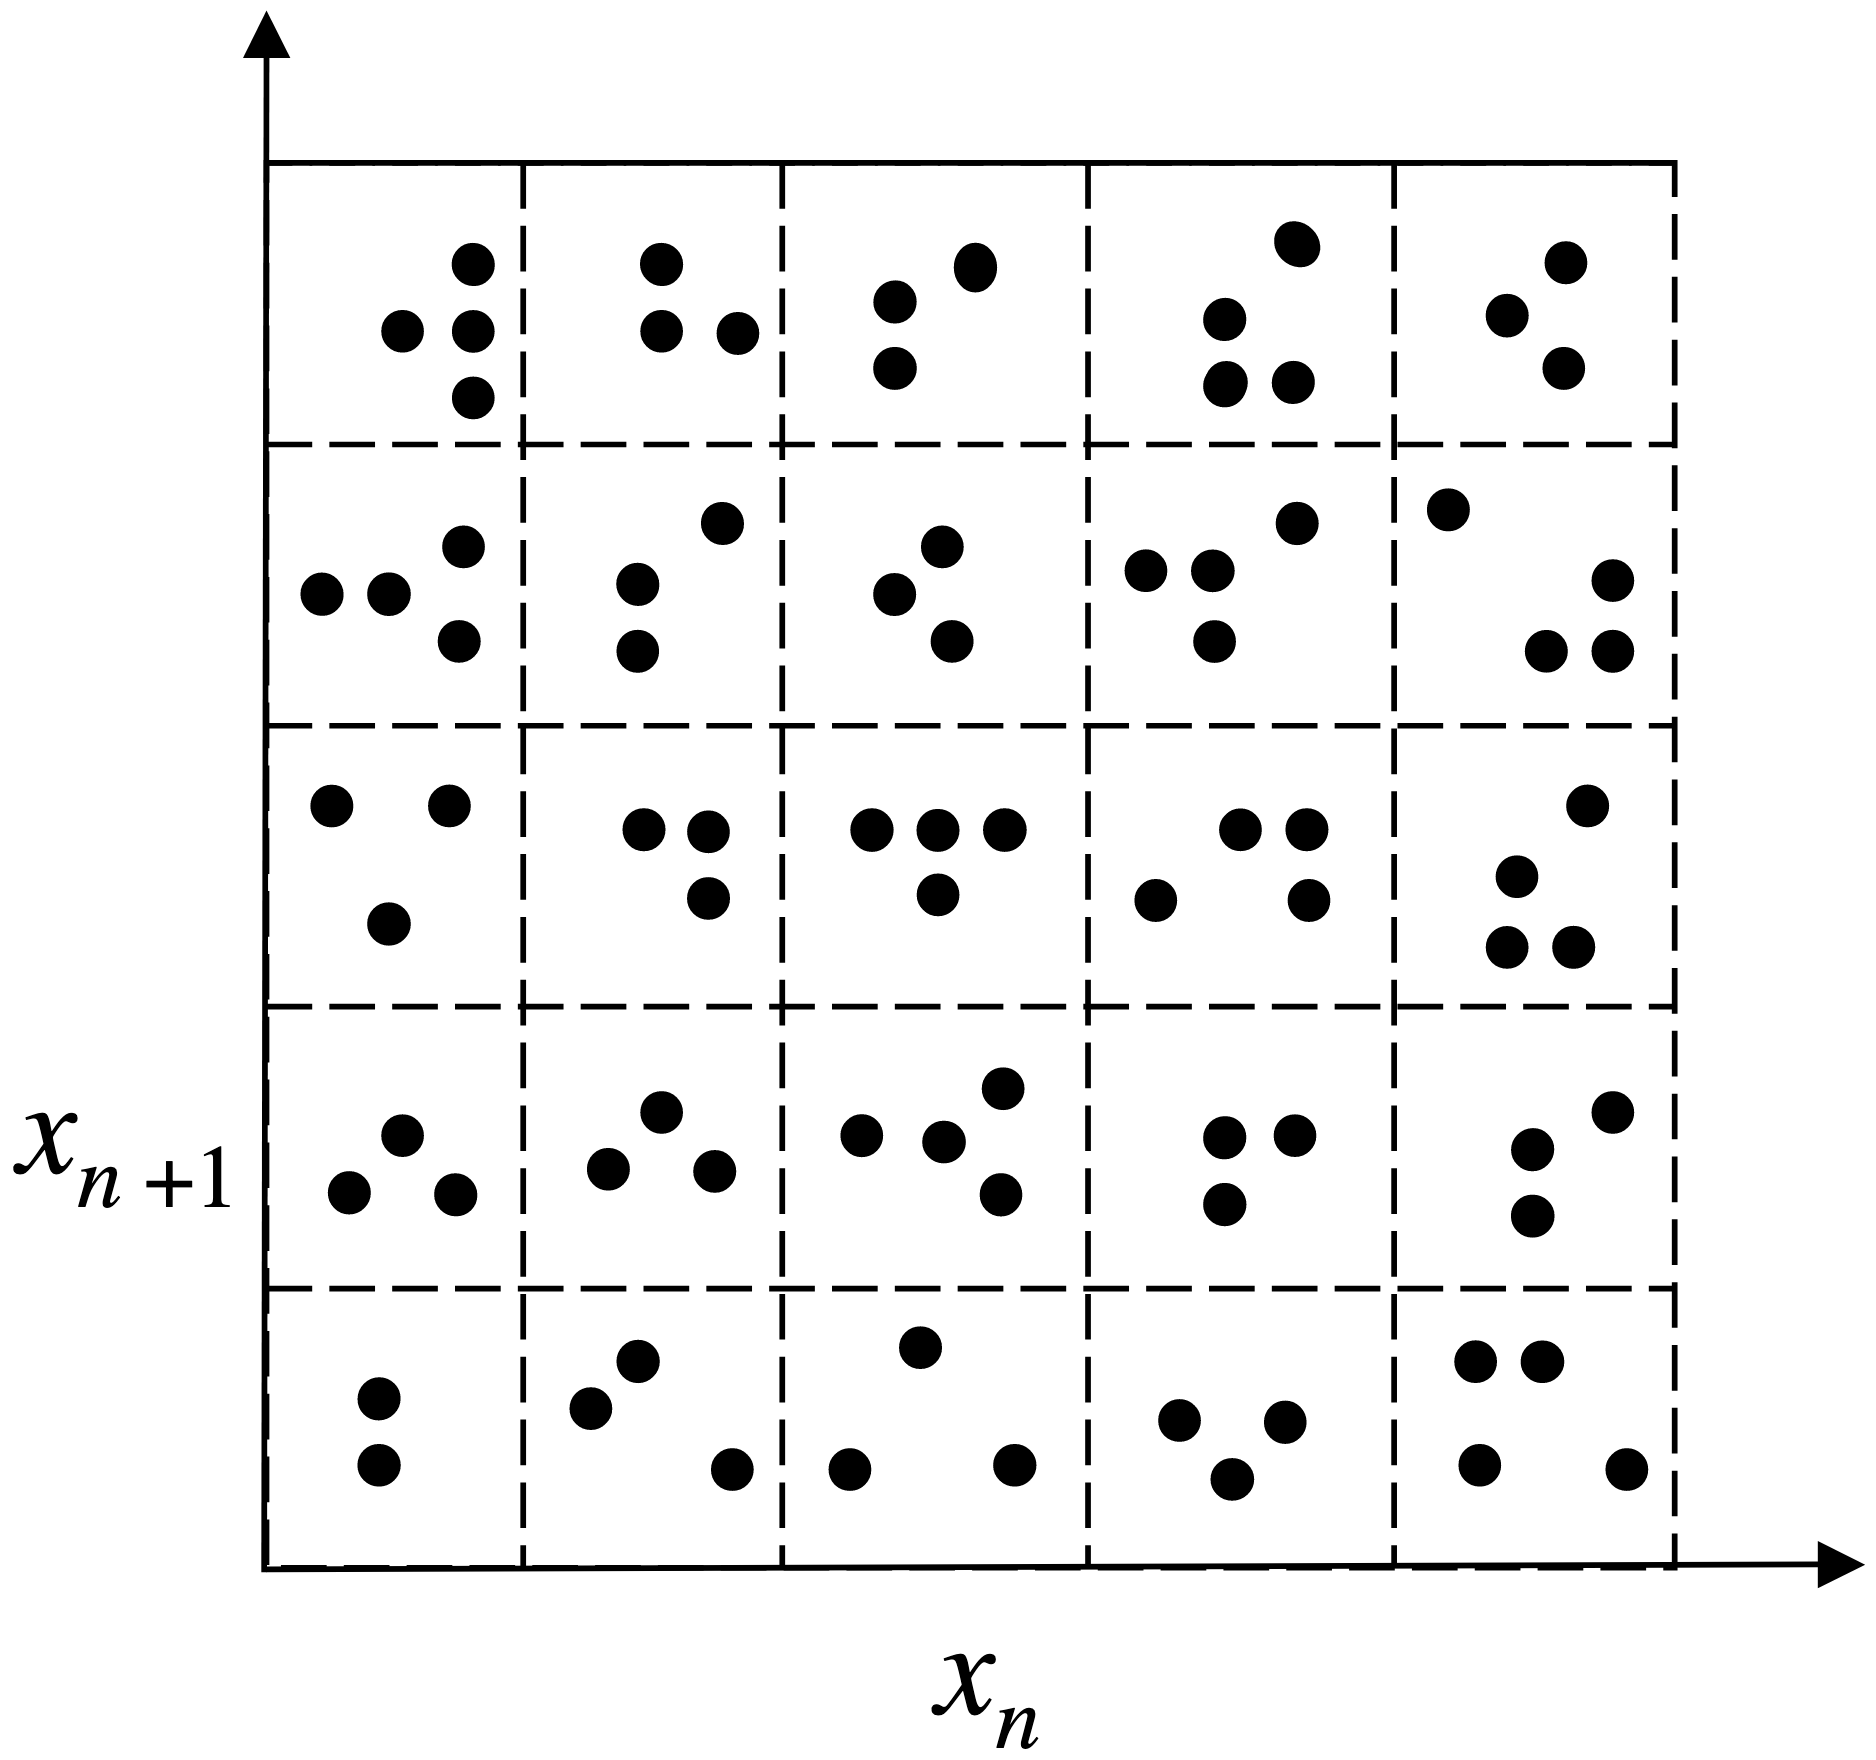
\includegraphics[width=0.5\linewidth]{inc/img/serial-test.png}
	\caption{Геометрический смысл критерия серий}
	\label{img:serial-test}
\end{figure}

Для каждой категории чисел $(q, r)$, где $0 \leqslant q, r < d$, подсчитываем количество случаев, когда пара $(X_{2j}, X_{2j + 1}) = (q, r)$ для $j = \overline{0, n - 1}$.
Затем применяем критерий хи-квадрат к этим $k = d^2$ категориям, с вероятностью $p = 1 / d^2$ отнесения пары чисел к каждой из категорий.

В критерии хи-квадрат вычисляется статистика
\begin{equation}
	\label{eqn:chi-squared}
	\chi^2 = \sum_{i = 0}^{k - 1} \frac{(Y_i - np_i)^2}{np_i},
\end{equation}
где $n$ — число независимых наблюдений, $p_i$ — вероятность того, что наблюдение относится к категории $i$, $Y_i$ — число наблюдений, которые относятся к категории $i$, при этом:
\begin{equation}
	\sum_{i = 0}^{k - 1} Y_i = n, \quad \sum_{i = 0}^{k - 1} p_i = 1.
\end{equation}

С учётом также $p_0 = p_1 = \ldots = p_{k - 1} = p$, формулу \eqref{eqn:chi-squared} можно преобразовать:
\begin{equation}
	\chi^2 = \frac pn \sum_{i = 0}^{k - 1} Y_i^2 - n.
\end{equation}

Число степеней свободы $\nu$ статистики хи-квадрат на единицу меньше числа категорий $k$.

Далее значение статистики сравнивается с приемлемым (табличным).
Если значение $\chi^2$ много больше или много меньше табличного, то гипотеза о равномерности случайной величины не выполняется, т. к. разброс чисел слишком велик или мал соответственно.
Если значение $\chi^2$ лежит между теоретическими значениями двух рядом стоящих столбцов —  гипотеза о равномерности случайной величины выполняется с вероятностью $p$, которая, в идеале, должна стремиться к 50 \%, но хорошим считается результат 5 — 95 \%.

\begin{table}[H]
	\centering
	\caption{Некоторые процентные точки $\chi^2$-распределения}
	\label{tbl:chi-squared}
	\begin{tabular}{|l|l|l|l|}
		\hline
		            & $\nu = 99$ & $\nu = 8099$ & $\nu = 809999$ \\ \hline
		$p = 0,999$ & 61,137     & 7711,395     & 806071,478     \\ \hline
		$p = 0,995$ & 66,510     & 7774,928     & 806724,263     \\ \hline
		$p = 0,99$  & 69,230     & 7805,867     & 807040,986     \\ \hline
		$p = 0,975$ & 73,361     & 7851,452     & 807506,270     \\ \hline
		$p = 0,95$  & 77,046     & 7890,800     & 807906,582     \\ \hline
		$p = 0,75$  & 89,181     & 8012,797     & 809140,152     \\ \hline
		$p = 0,5$   & 98,334     & 8098,333     & 809998,333     \\ \hline
		$p = 0,25$  & 108,093    & 8184,476     & 810857,121     \\ \hline
		$p = 0,05$  & 123,225    & 8309,474     & 812093,692     \\ \hline
		$p = 0,025$ & 128,422    & 8350,336     & 812495,519     \\ \hline
		$p = 0,01$  & 134,642    & 8398,015     & 812962,897     \\ \hline
		$p = 0,005$ & 138,987    & 8430,585     & 813281,250     \\ \hline
		$p = 0,001$ & 148,230    & 8498,004     & 813937,922     \\ \hline
	\end{tabular}
\end{table}

\chapter{Результат работы}

Для исследования генераторов псевдослучайных чисел алгоритмическим методом было сгенерировано по $2\,000\,000$ одно-, двух- и трёх-разрядных чисел, табличным методом — по $150\,000$ чисел.

\begin{figure}[H]
	\centering
	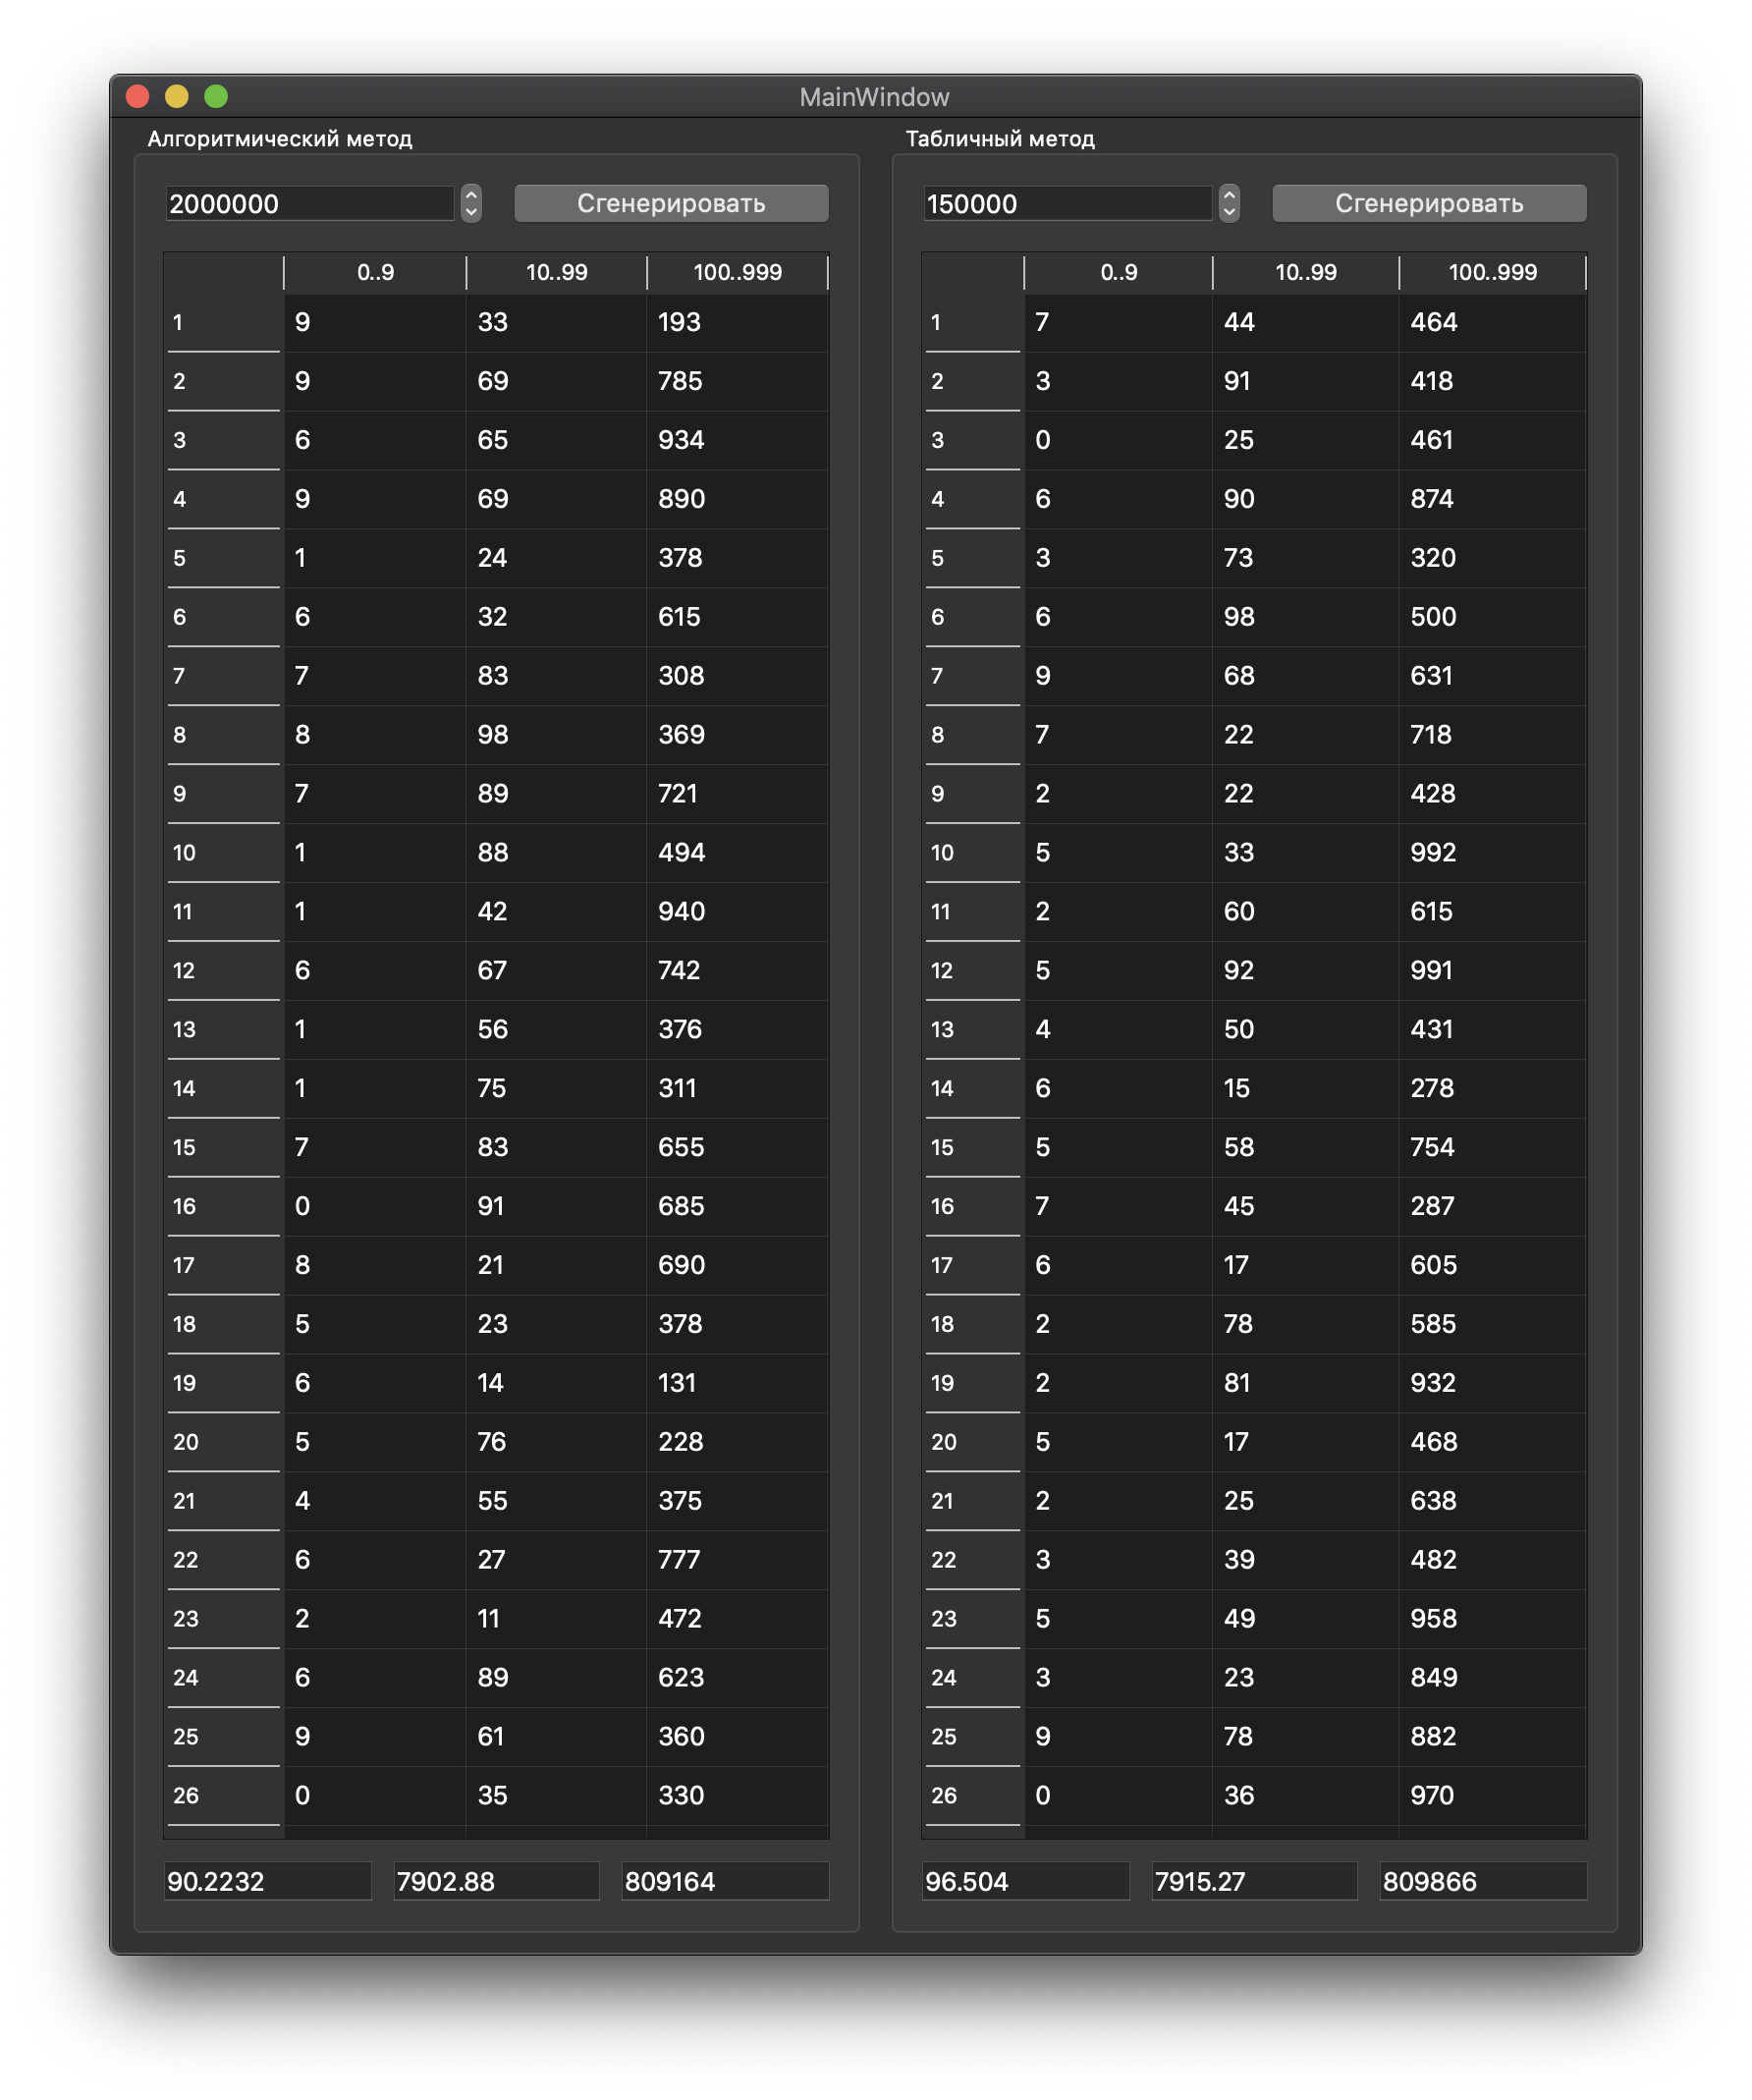
\includegraphics[width=0.99\linewidth]{inc/img/result.png}
	\caption{Результат работы программы}
	\label{img:result}
\end{figure}

\chapter*{Вывод}
\addcontentsline{toc}{chapter}{Вывод}

Рассмотрены алгоритмический (MT19937) и табличный генераторы псевдослучайных чисел.
Оба метода удовлетворяют критерию серий — получают оценку 5 — 95 \%, а именно:

\begin{table}[H]
	\centering
	\caption{Оценка ГПСЧ}
	\begin{tabular}{|c|c|c|c|}
		\hline
		                               & \textbf{0..9}   & \textbf{10..99} & \textbf{100..999} \\ \hline
		\textbf{Алгоритмический метод} & $p = 72,422$ \% & $p = 93,923$ \% & $p = 74,400$ \%   \\ \hline
		\textbf{Табличный метод}       & $p = 55,227$ \% & $p = 92,639$ \% & $p = 54,141$ \%   \\ \hline
	\end{tabular}
\end{table}

Достоинством данных методов является быстродействие и генерация качественных псевдослучайных чисел.
Хороший результат табличного ГПСЧ обусловлен тем, что в таблице содержатся проверенные некоррелированные цифры.
В то же время, для хранения большого количества цифр, от которого зависит период генератора, требуется много памяти.

Алгоритм MT19937 этих недостатков лишён, его период составляет практически недостижимые $2^{19937} - 1$, однако по качеству генерируемых чисел немного уступает табличному методу.


\end{document}
